%!Tex TS-program = xelatex
\documentclass[10pt]{article}
\usepackage[paperwidth=7in,paperheight=9in,margin=0.3in]{geometry}
\usepackage{xcolor}
\usepackage{fontspec}
\usepackage{booktabs}
\usepackage{array}
\usepackage{multirow}
\usepackage{colortbl}
\usepackage{titlesec}
\usepackage{parskip}
\usepackage{setspace}
\usepackage{enumitem}
\usepackage{graphicx}
\usepackage{subcaption}
\usepackage{float}

% Font configuration
\setmainfont{QTBookmann}
\setmonofont{VictorMono Nerd Font}[Scale=0.85]

% Colors optimized for e-reader
\definecolor{primary}{RGB}{0, 0, 0}
\definecolor{secondary}{RGB}{60, 60, 60}
\definecolor{accent}{RGB}{150, 0, 0}
\definecolor{tableheader}{RGB}{230, 230, 230}
\definecolor{rowlight}{RGB}{248, 248, 248}
\definecolor{rowdark}{RGB}{240, 240, 240}
\definecolor{targetcolor}{RGB}{220, 240, 220}

% Section formatting
\titleformat{\section}
  {\fontspec{QTBookmann}\Large\bfseries\color{primary}}
  {}{0em}{}
\titleformat{\subsection}
  {\fontspec{QTBookmann}\large\bfseries\color{accent}}
  {}{0em}{}
\titleformat{\subsubsection}
  {\fontspec{QTBookmann}\normalsize\bfseries\color{secondary}}
  {}{0em}{}

% Compact itemize
\setlist[itemize]{leftmargin=*,topsep=2pt,itemsep=1pt}
\setlength{\parskip}{2pt}
\setstretch{1.05}

\begin{document}

\section*{Movie Production Analytics Dataset}
{\color{secondary}\noindent\textbf{500 Films • 19 Features • Dual Target Analysis}}

\vspace{4pt}
\noindent{\color{secondary}\small Comprehensive dataset for predicting commercial success and technical award outcomes.}

\vspace{8pt}

\subsection*{📊 Dataset Profile}
\begin{minipage}[t]{0.48\textwidth}
\begin{itemize}
  \item \textbf{Records:} 500 films
  \item \textbf{Features:} 19 variables
  \item \textbf{Timeframe:} Modern era
  \item \textbf{Completeness:} 99.8\%
\end{itemize}
\end{minipage}
\hfill
\begin{minipage}[t]{0.48\textwidth}
\begin{itemize}
  \item \textbf{Target 1:} Box office revenue
  \item \textbf{Target 2:} Technical award
  \item \textbf{Genres:} 4 primary categories
  \item \textbf{Quality:} Analysis-ready
\end{itemize}
\end{minipage}

\vspace{8pt}

\subsection*{🎯 Target Variables}
\begin{tabular}{>{\ttfamily}l>{\raggedright\arraybackslash}p{2cm}>{\raggedright\arraybackslash}p{3cm}>{\raggedright\arraybackslash}p{2.5cm}}
\toprule
\rowcolor{tableheader}
\textbf{Variable} & \textbf{Type} & \textbf{Purpose} & \textbf{Range/Values} \\
\midrule
Collection & Continuous & Box office revenue & 10,000 - 100,000 \\
Start\_Tech\_Oscar & Binary & Award achievement & 0 (No), 1 (Yes) \\
\bottomrule
\end{tabular}

\vspace{8pt}

\subsection*{💰 Financial Features}
{\rowcolors{2}{rowlight}{rowdark}
\begin{tabular}{>{\ttfamily}l>{\raggedright\arraybackslash}p{1.8cm}>{\raggedright\arraybackslash}p{2.8cm}>{\raggedright\arraybackslash}p{2cm}>{\raggedright\arraybackslash}p{1.8cm}}
\toprule
\rowcolor{tableheader}
\textbf{Feature} & \textbf{Type} & \textbf{Description} & \textbf{Range} & \textbf{Impact} \\
\midrule
Marketing\_expense & Continuous & Promotion budget & 20-1,799k & High \\
Production\_expense & Continuous & Physical production cost & 57-106 & Medium \\
Budget & Continuous & Total project financing & 19k-48k & High \\
Num\_multiplex & Discrete & Theater count & 347-868 & High \\
Multiplex\_coverage & Continuous & Distribution percentage & 0.12-0.61 & High \\
\bottomrule
\end{tabular}

\vspace{8pt}

\subsection*{🎬 Creative Features}
{\rowcolors{2}{rowlight}{rowdark}
\begin{tabular}{>{\ttfamily}l>{\raggedright\arraybackslash}p{1.8cm}>{\raggedright\arraybackslash}p{2.8cm}>{\raggedright\arraybackslash}p{2cm}>{\raggedright\arraybackslash}p{1.8cm}}
\toprule
\rowcolor{tableheader}
\textbf{Feature} & \textbf{Type} & \textbf{Description} & \textbf{Range} & \textbf{Impact} \\
\midrule
Movie\_length & Continuous & Runtime in minutes & 76-217 & Medium \\
Genre & Categorical & Film category & 4 types & High \\
Avg\_age\_actors & Discrete & Cast average age & 20-60 & Low \\
Lead\_Actor\_Rating & Continuous & Performance score & 3.8-9.5 & High \\
Lead\_Actress\_rating & Continuous & Performance score & 4.0-9.5 & High \\
Director\_rating & Continuous & Director quality & 3.8-9.6 & High \\
Producer\_rating & Continuous & Producer quality & 4.0-9.6 & Medium \\
Critic\_rating & Continuous & Professional reviews & 3.8-9.4 & High \\
\bottomrule
\end{tabular}

\vspace{8pt}

\subsection*{📢 Marketing \& Technical Features}
{\rowcolors{2}{rowlight}{rowdark}
\begin{tabular}{>{\ttfamily}l>{\raggedright\arraybackslash}p{1.8cm}>{\raggedright\arraybackslash}p{2.8cm}>{\raggedright\arraybackslash}p{2cm}>{\raggedright\arraybackslash}p{1.8cm}}
\toprule
\rowcolor{tableheader}
\textbf{Feature} & \textbf{Type} & \textbf{Description} & \textbf{Range} & \textbf{Impact} \\
\midrule
Trailer\_views & Discrete & Online preview popularity & 215k-567k & High \\
3D\_available & Binary & 3D format availability & Yes/No & Medium \\
Time\_taken & Continuous & Production duration & 0-217 days & Low \\
Twitter\_hastags & Continuous & Social media engagement & 200-1,600+ & Medium \\
\bottomrule
\end{tabular}

\vspace{8pt}

\subsection*{📈 Comprehensive Feature Analysis}

\subsubsection*{Financial Features Analysis}

\begin{figure}[H]
\centering
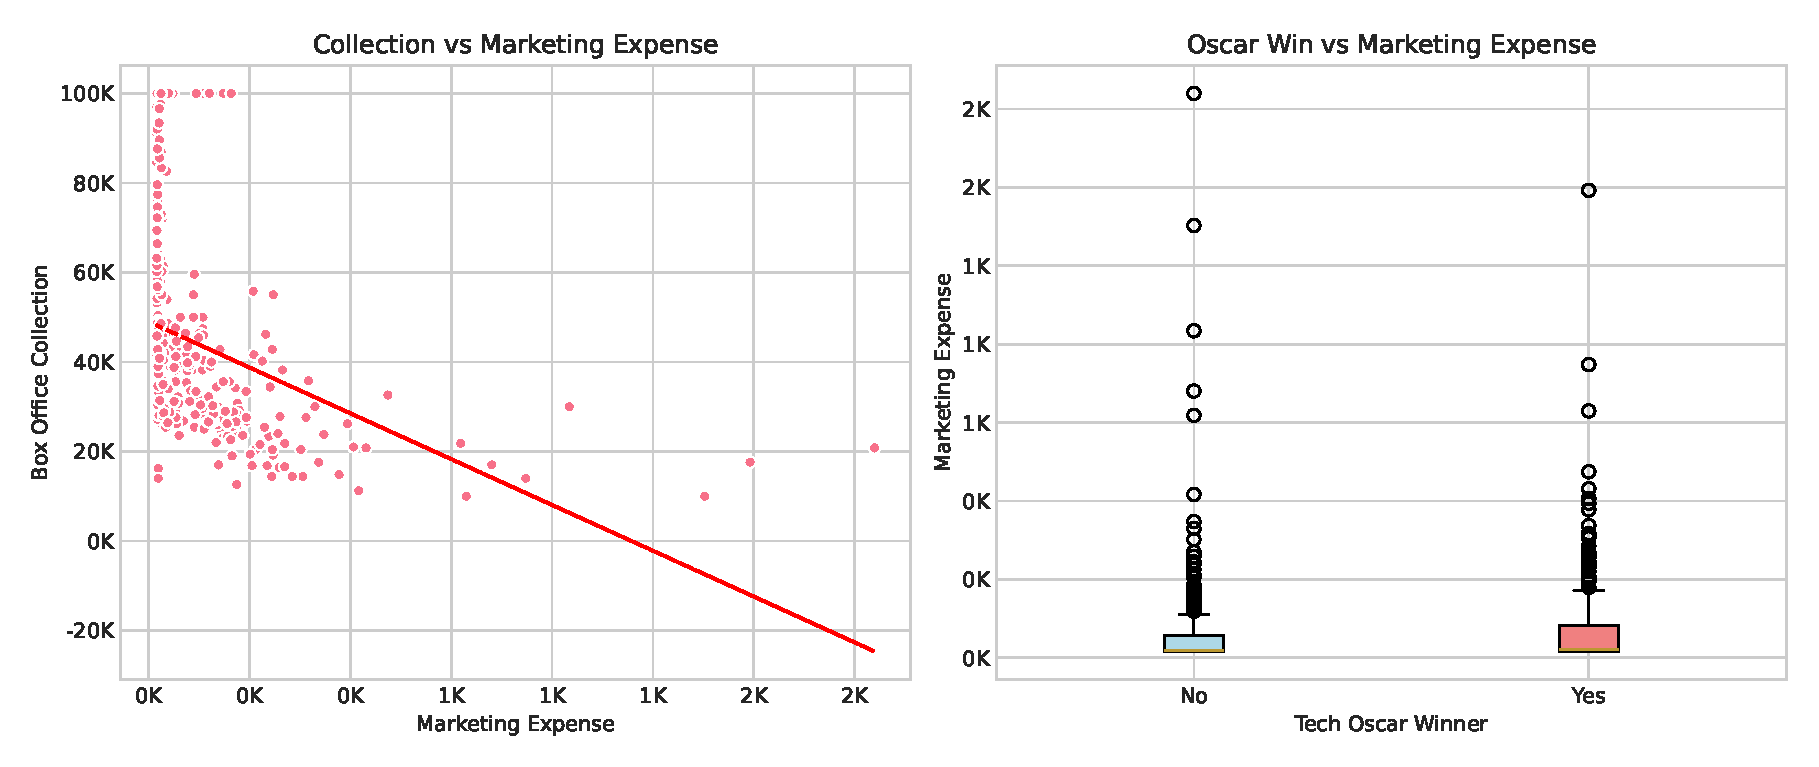
\includegraphics[width=0.85\textwidth]{../DatasetAnalysis/plots/Marketing_expense.eps}
\caption{Marketing Expense vs Targets: Strong positive correlation with Collection, moderate differentiation for Oscar wins.}
\end{figure}

\begin{figure}[H]
\centering
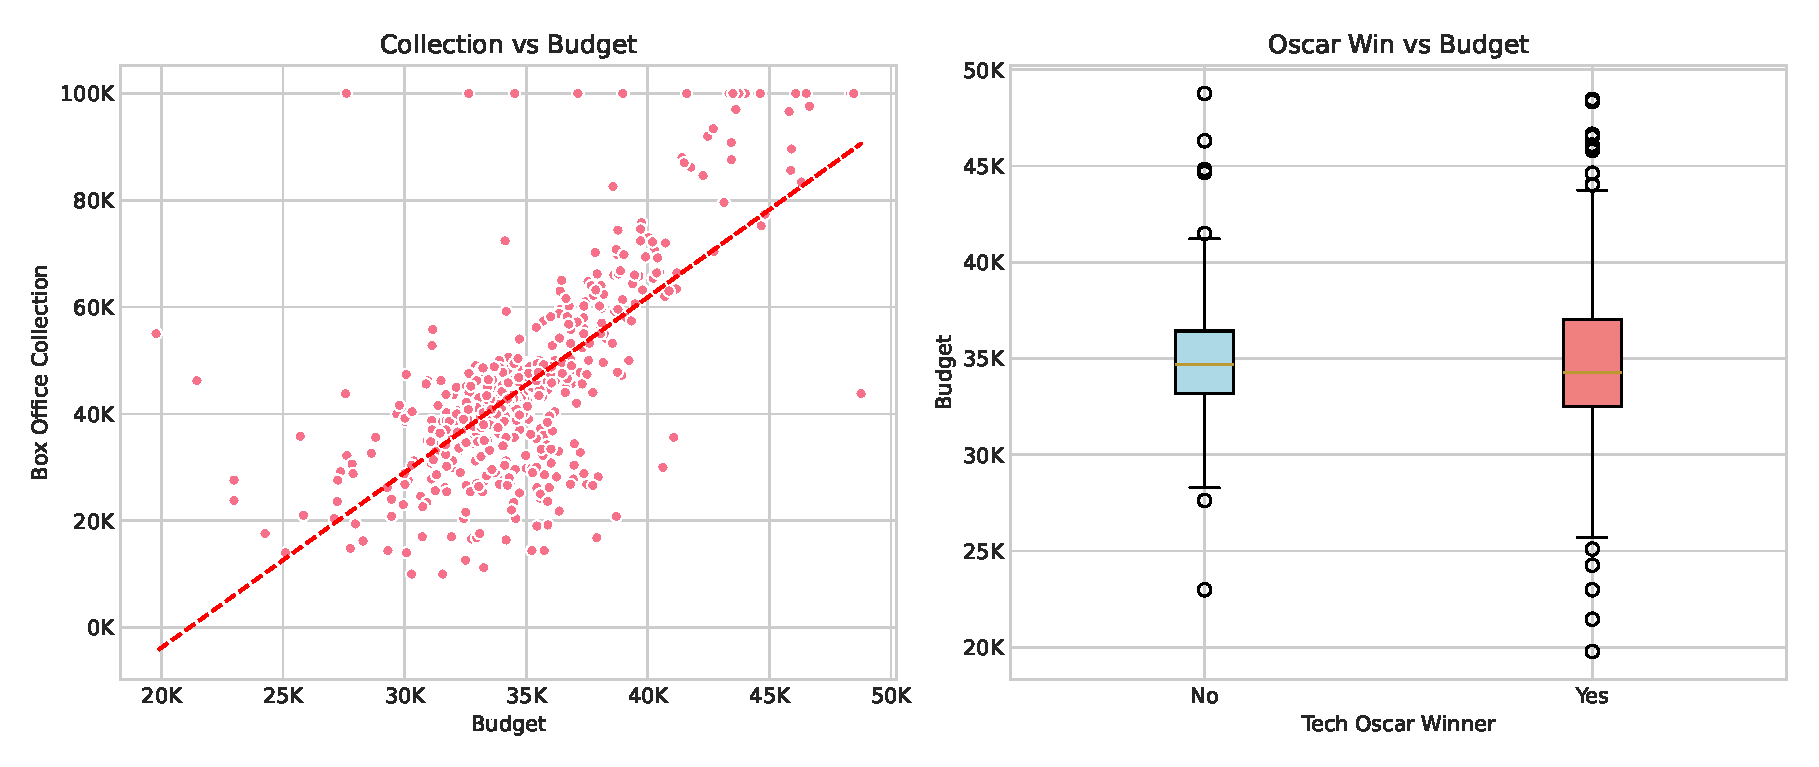
\includegraphics[width=0.85\textwidth]{../DatasetAnalysis/plots/Budget.eps}
\caption{Budget vs Targets: Clear linear relationship with Collection, significant budget difference for Oscar winners.}
\end{figure}

\begin{figure}[H]
\centering
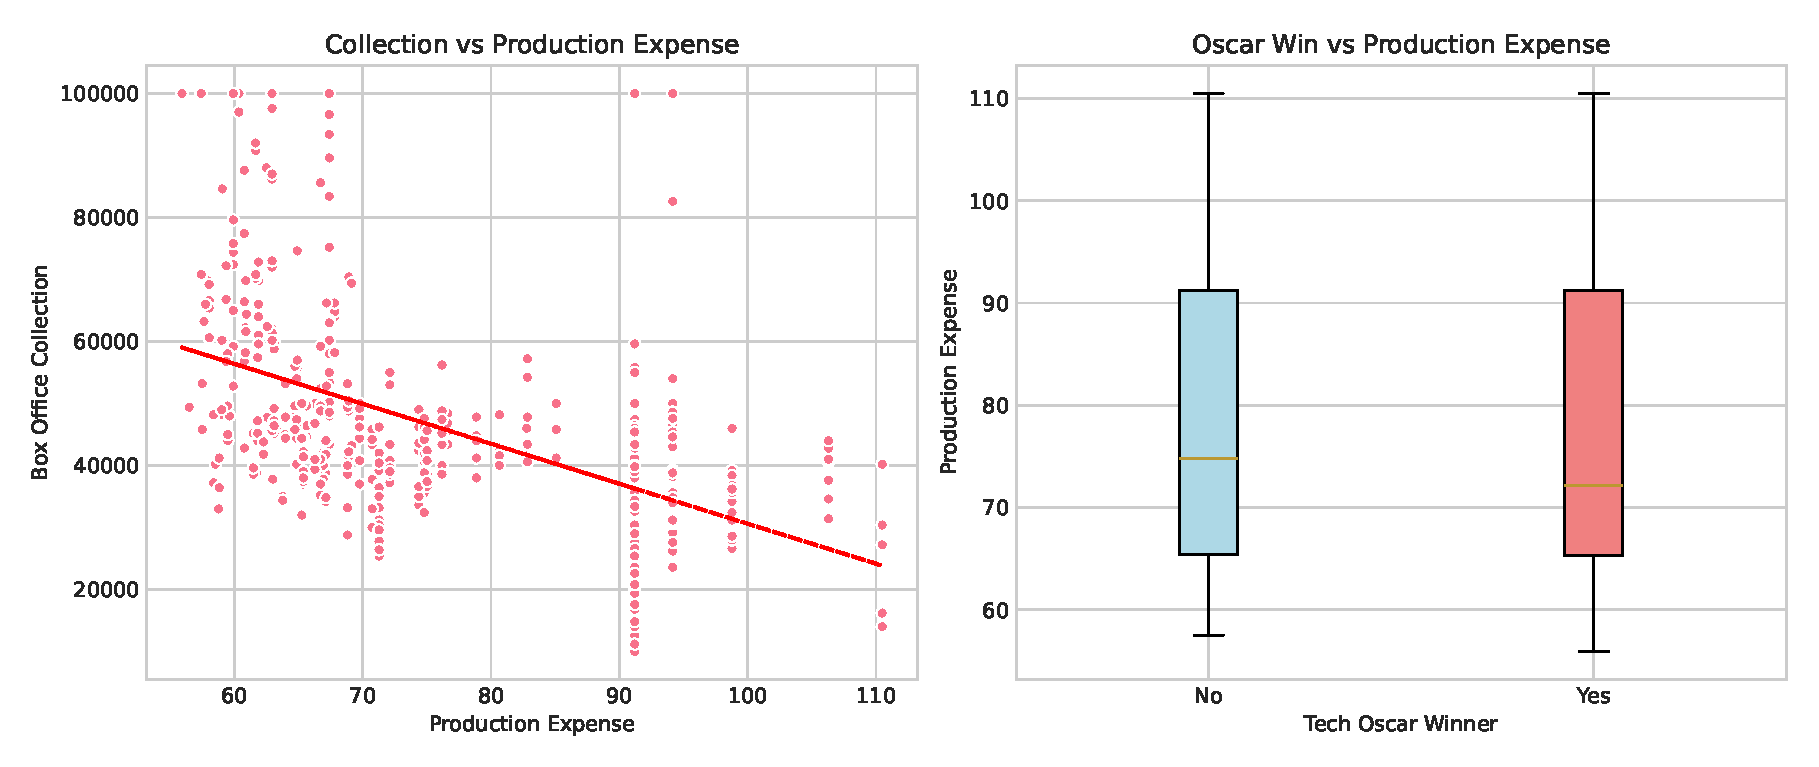
\includegraphics[width=0.85\textwidth]{../DatasetAnalysis/plots/Production_expense.eps}
\caption{Production Expense vs Targets: Clustered distribution shows standardized production costs across films.}
\end{figure}

\subsubsection*{Distribution \& Release Features}

\begin{figure}[H]
\centering
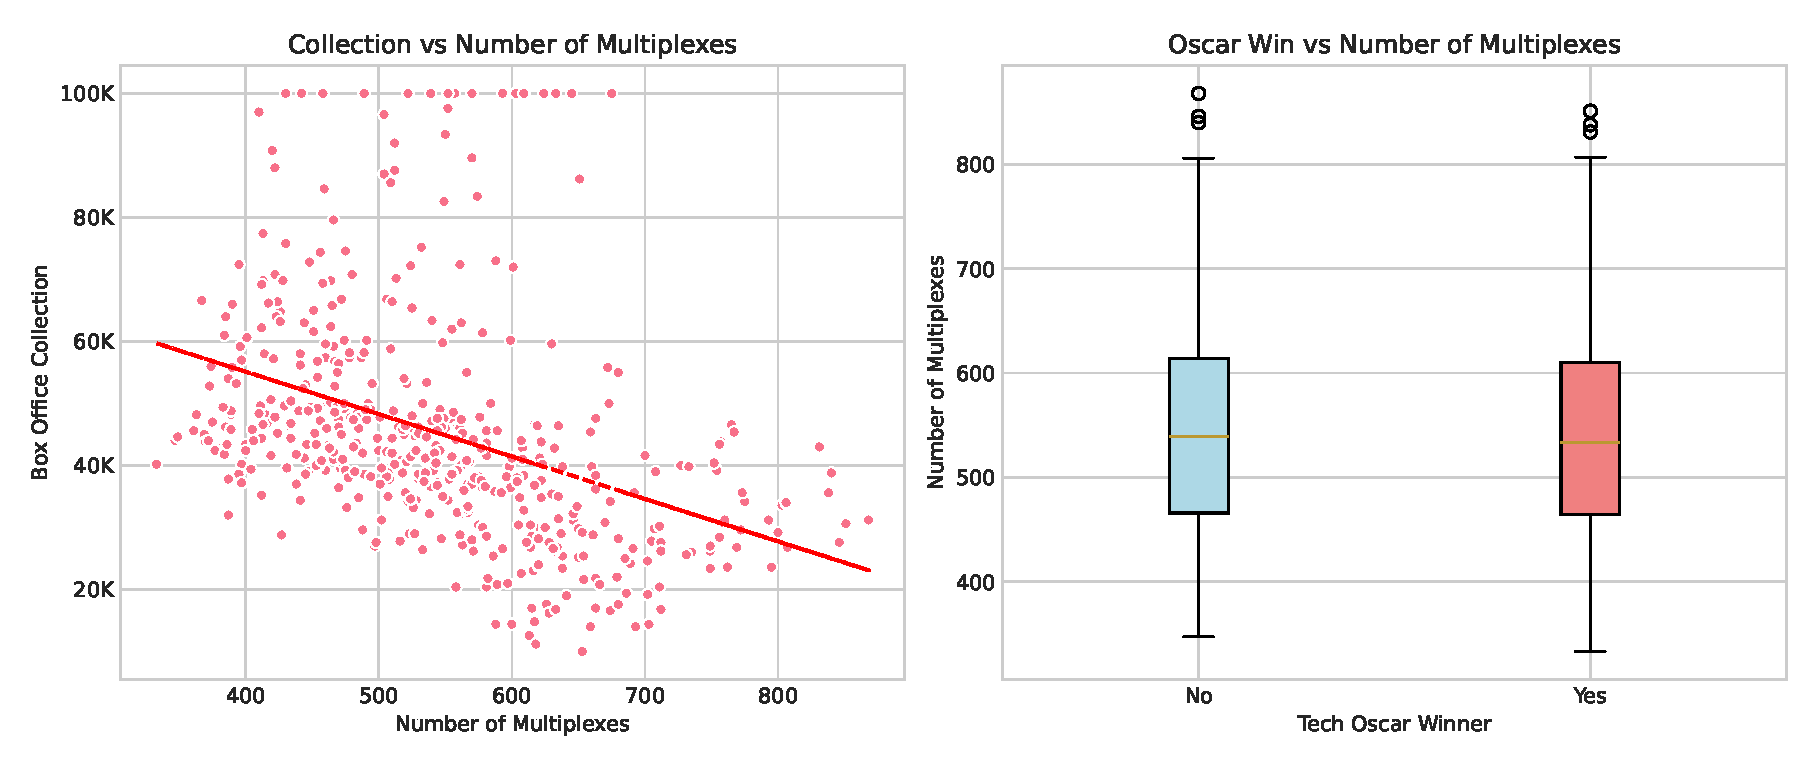
\includegraphics[width=0.85\textwidth]{../DatasetAnalysis/plots/Num_multiplex.eps}
\caption{Number of Multiplexes vs Targets: Wide release strongly correlates with higher Collection.}
\end{figure}

\begin{figure}[H]
\centering
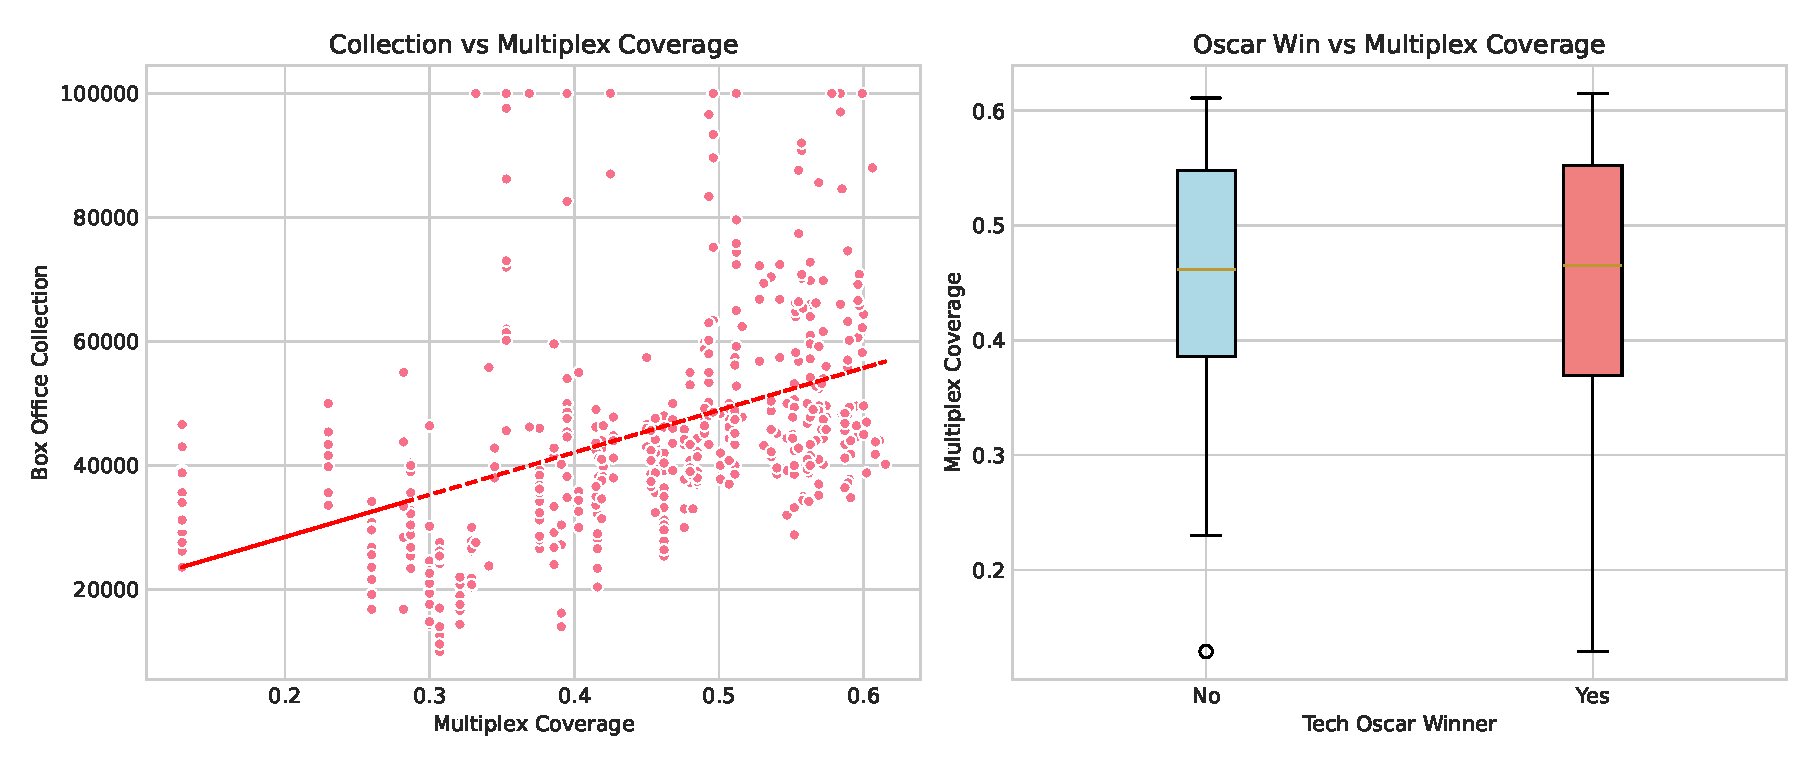
\includegraphics[width=0.85\textwidth]{../DatasetAnalysis/plots/Multiplex_coverage.eps}
\caption{Multiplex Coverage vs Targets: Distribution reach shows strong commercial impact.}
\end{figure}

\subsubsection*{Creative Team \& Quality Metrics}

\begin{figure}[H]
\centering
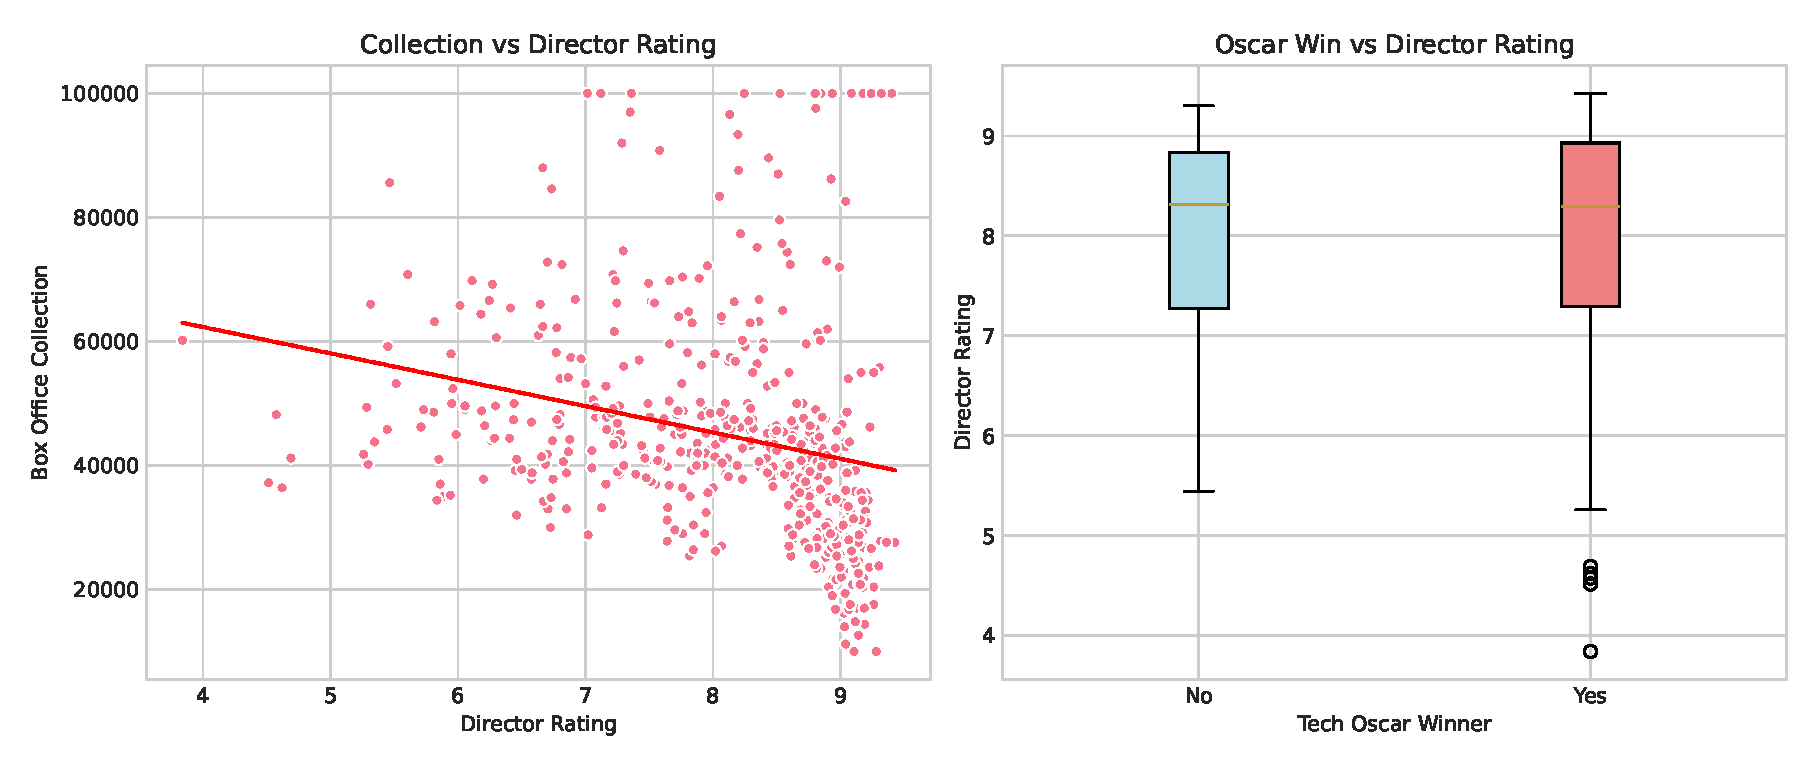
\includegraphics[width=0.85\textwidth]{../DatasetAnalysis/plots/Director_rating.eps}
\caption{Director Rating vs Targets: Critical factor for both commercial success and awards.}
\end{figure}

\begin{figure}[H]
\centering
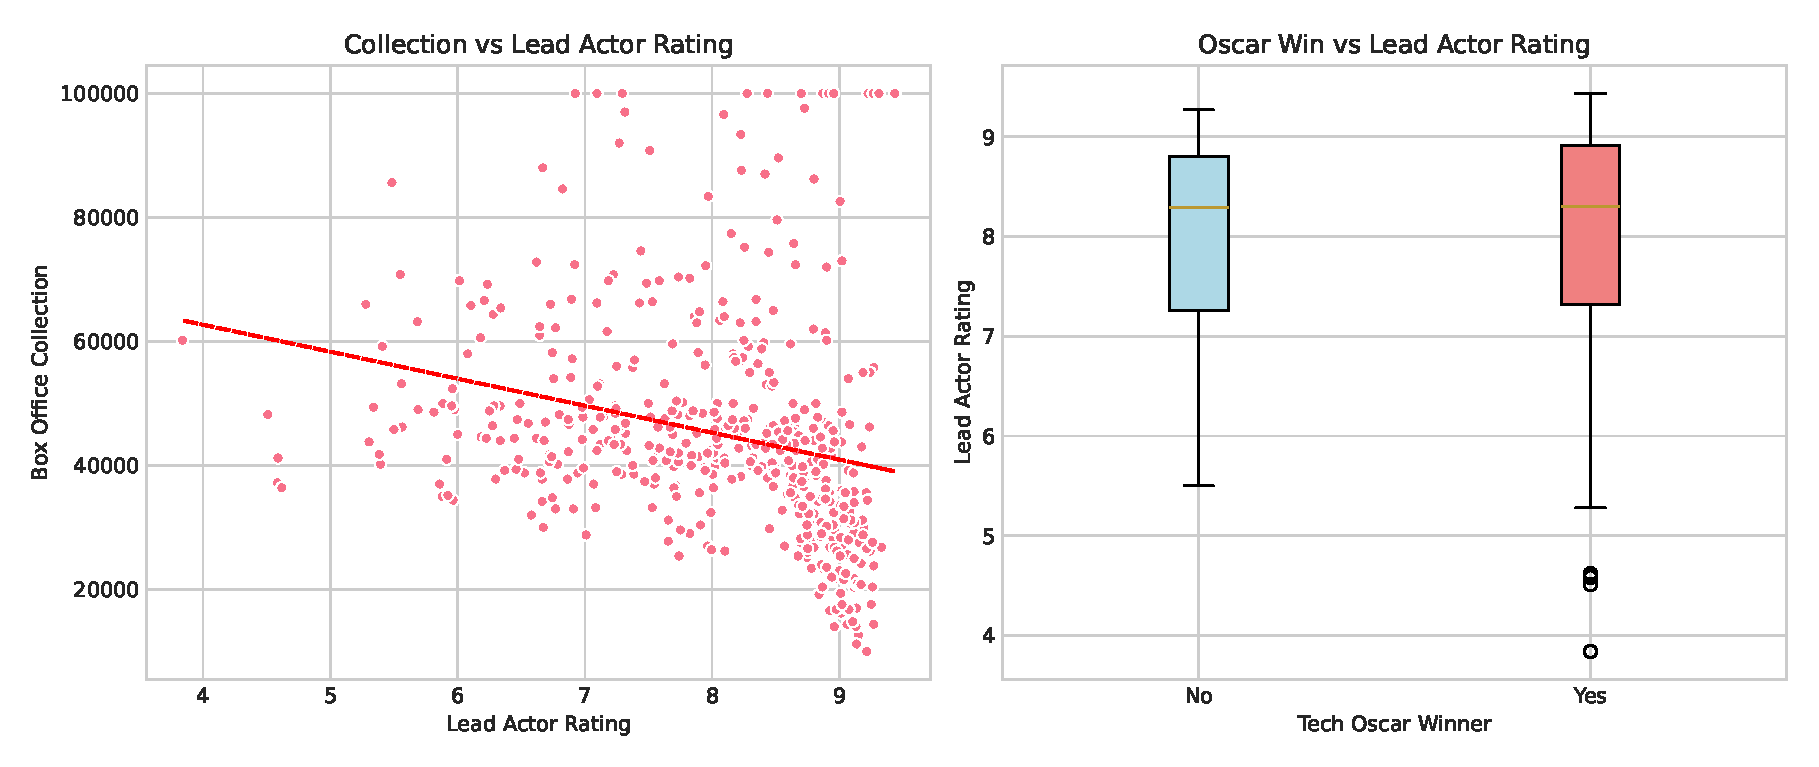
\includegraphics[width=0.85\textwidth]{../DatasetAnalysis/plots/Lead__Actor_Rating.eps}
\caption{Lead Actor Rating vs Targets: Star power influences Collection, less impact on technical awards.}
\end{figure}

\begin{figure}[H]
\centering
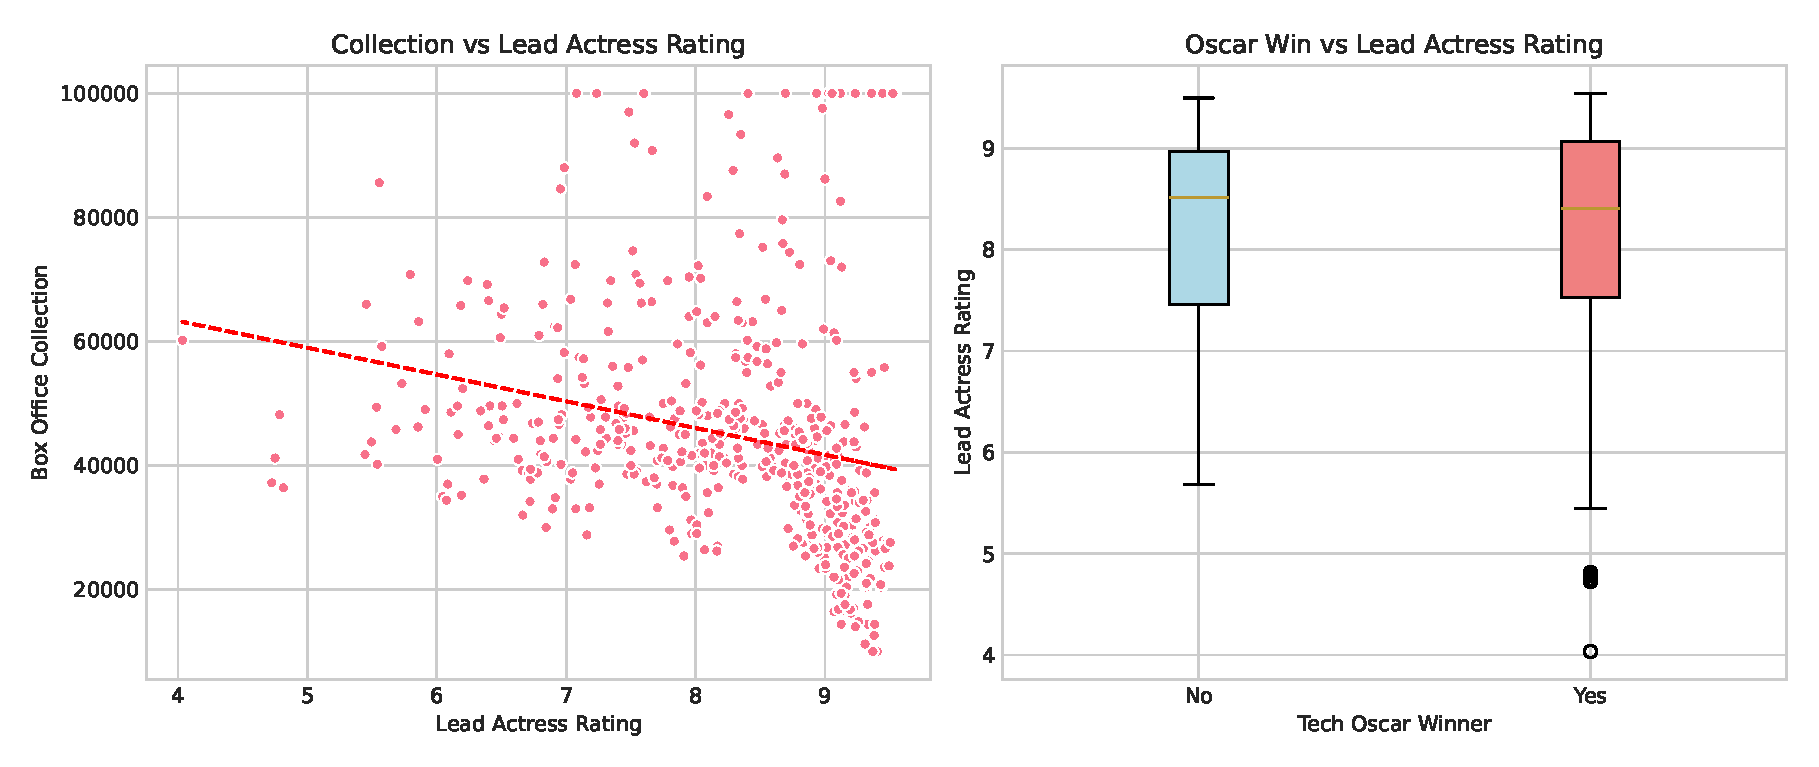
\includegraphics[width=0.85\textwidth]{../DatasetAnalysis/plots/Lead_Actress_rating.eps}
\caption{Lead Actress Rating vs Targets: Similar pattern to actor ratings with commercial focus.}
\end{figure}

\begin{figure}[H]
\centering
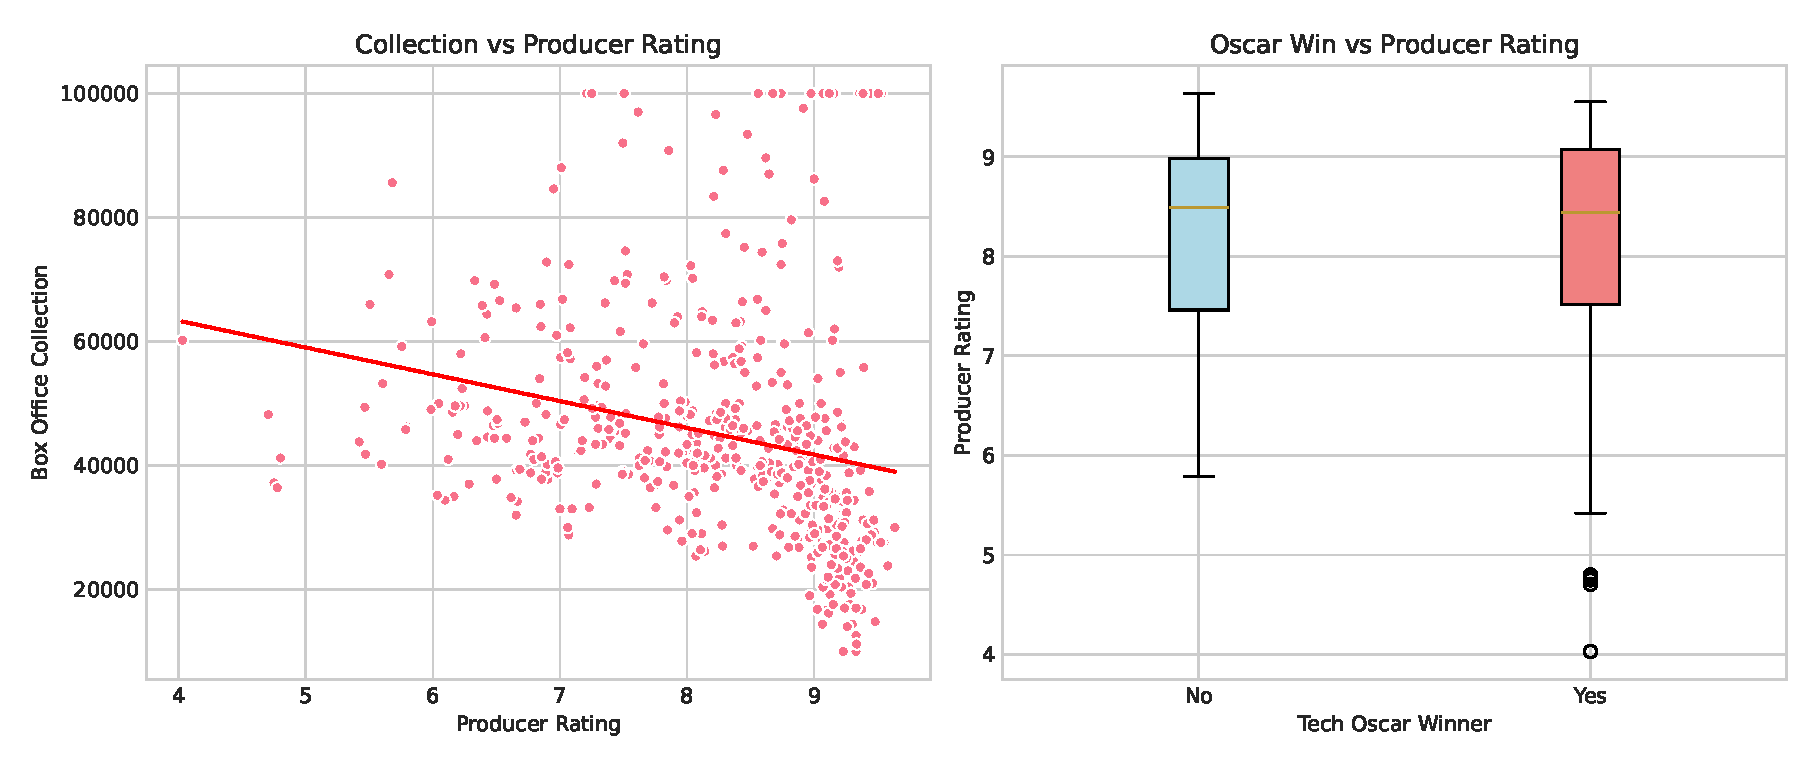
\includegraphics[width=0.85\textwidth]{../DatasetAnalysis/plots/Producer_rating.eps}
\caption{Producer Rating vs Targets: Production quality important for technical award consideration.}
\end{figure}

\begin{figure}[H]
\centering
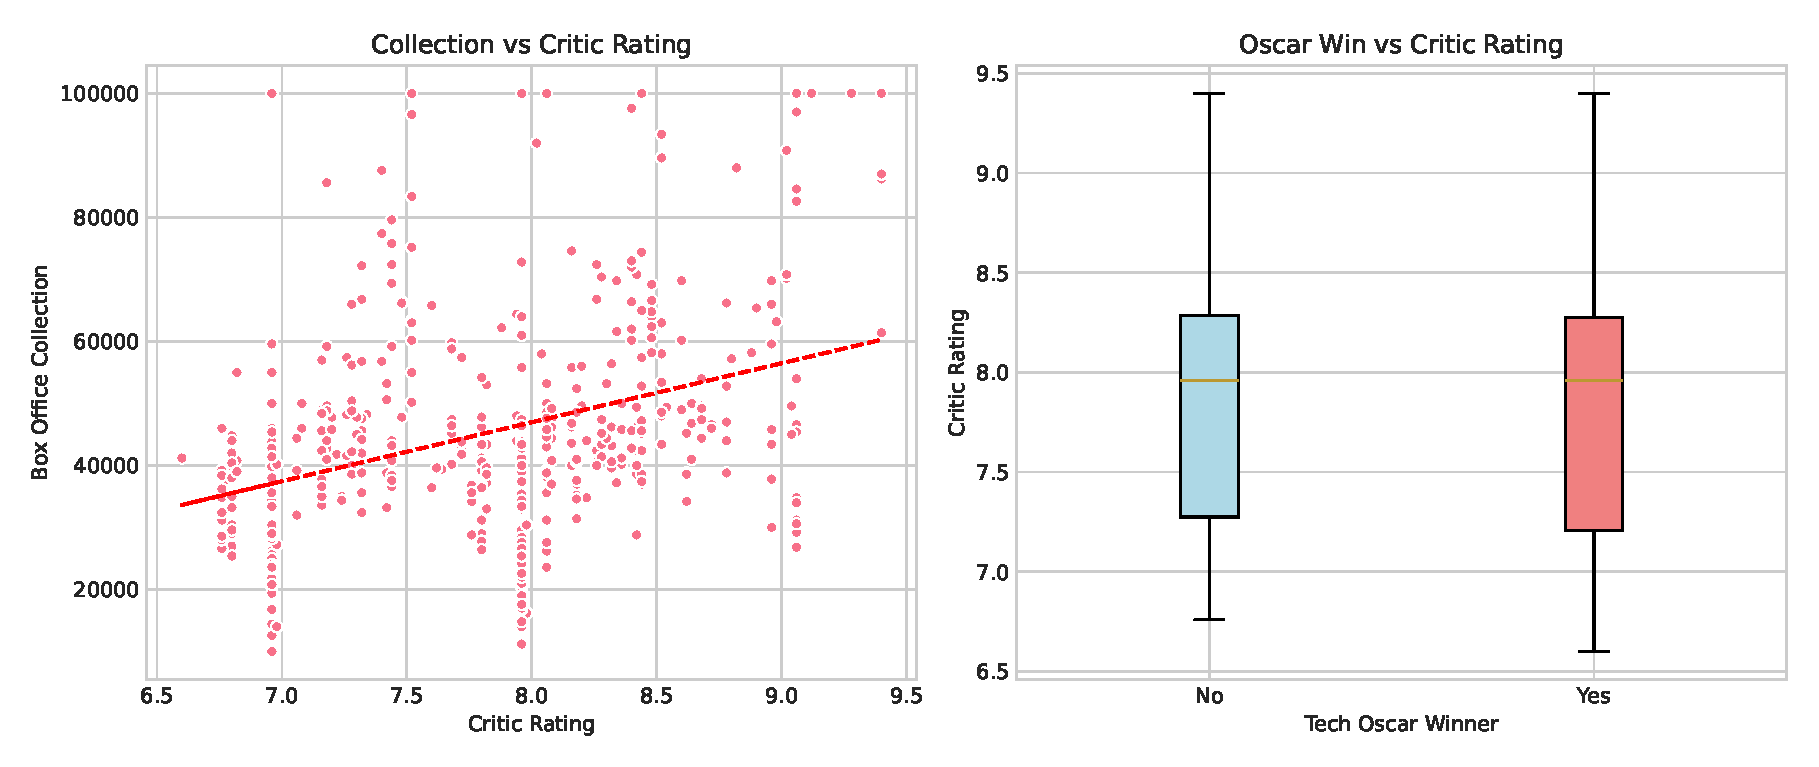
\includegraphics[width=0.85\textwidth]{../DatasetAnalysis/plots/Critic_rating.eps}
\caption{Critic Rating vs Targets: Critical acclaim correlates with both targets but stronger for awards.}
\end{figure}

\subsubsection*{Content \& Technical Features}

\begin{figure}[H]
\centering
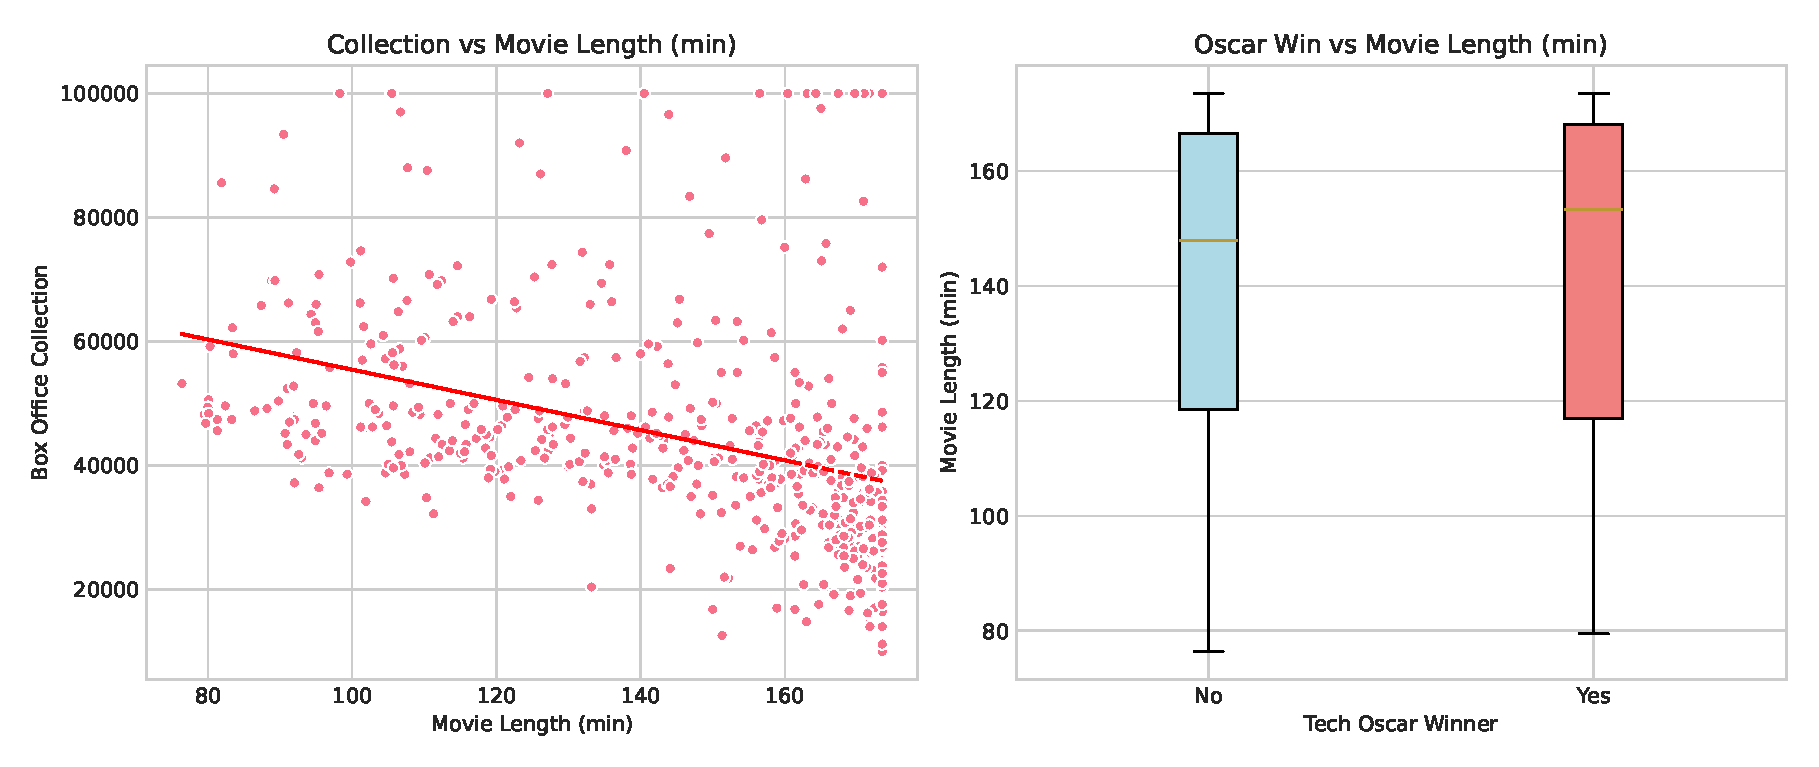
\includegraphics[width=0.85\textwidth]{../DatasetAnalysis/plots/Movie_length.eps}
\caption{Movie Length vs Targets: Runtime shows complex relationship with both commercial and critical success.}
\end{figure}

\begin{figure}[H]
\centering
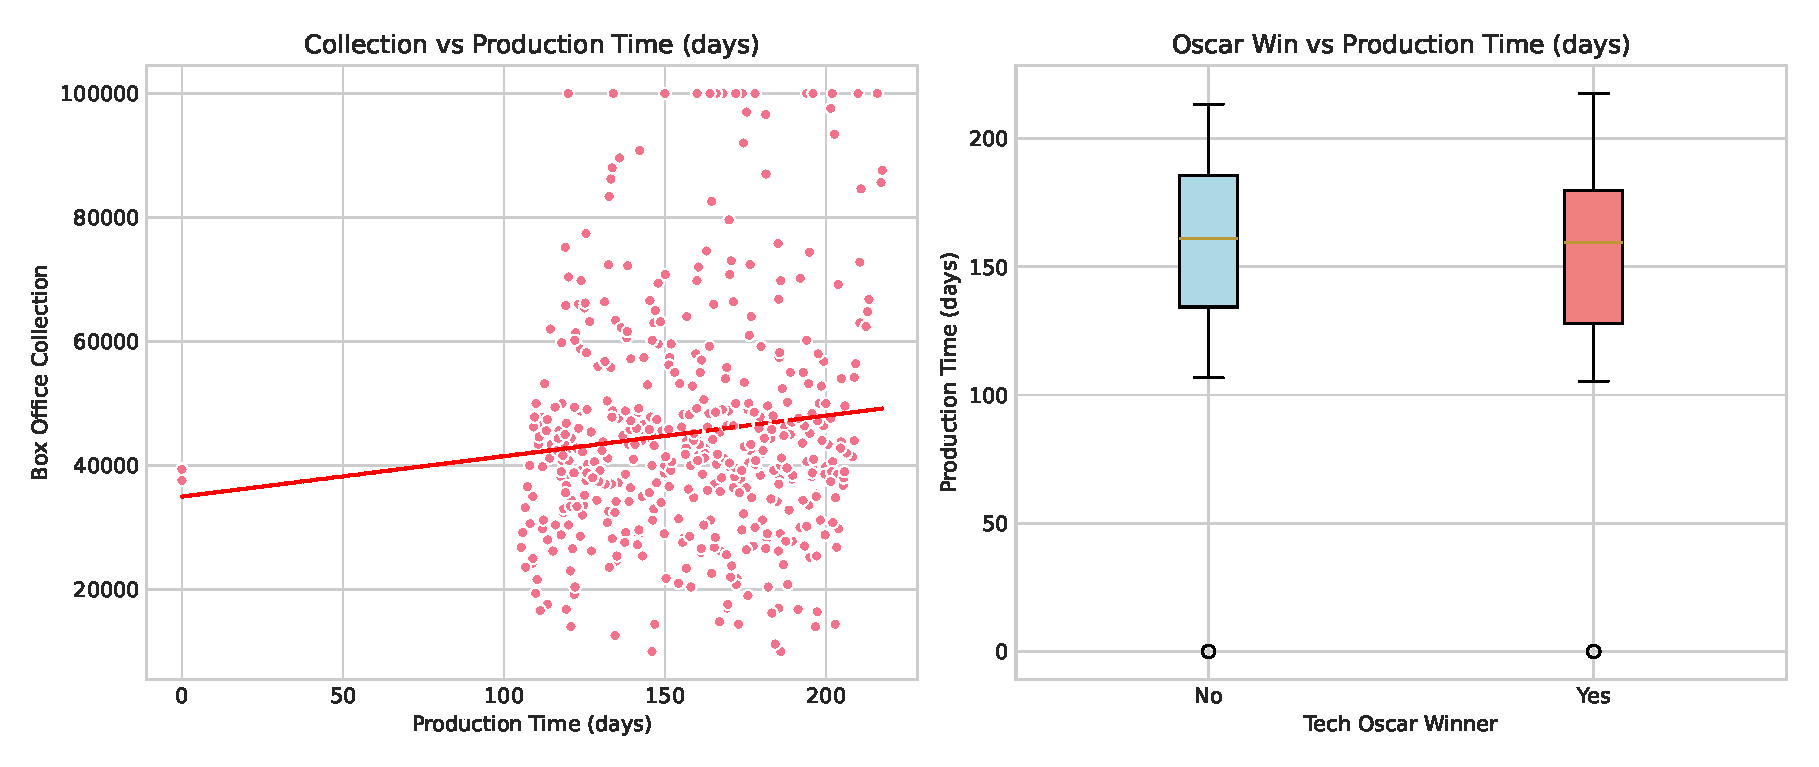
\includegraphics[width=0.85\textwidth]{../DatasetAnalysis/plots/Time_taken.eps}
\caption{Production Time vs Targets: Longer production doesn't guarantee better outcomes.}
\end{figure}

\subsubsection*{Marketing \& Audience Engagement}

\begin{figure}[H]
\centering
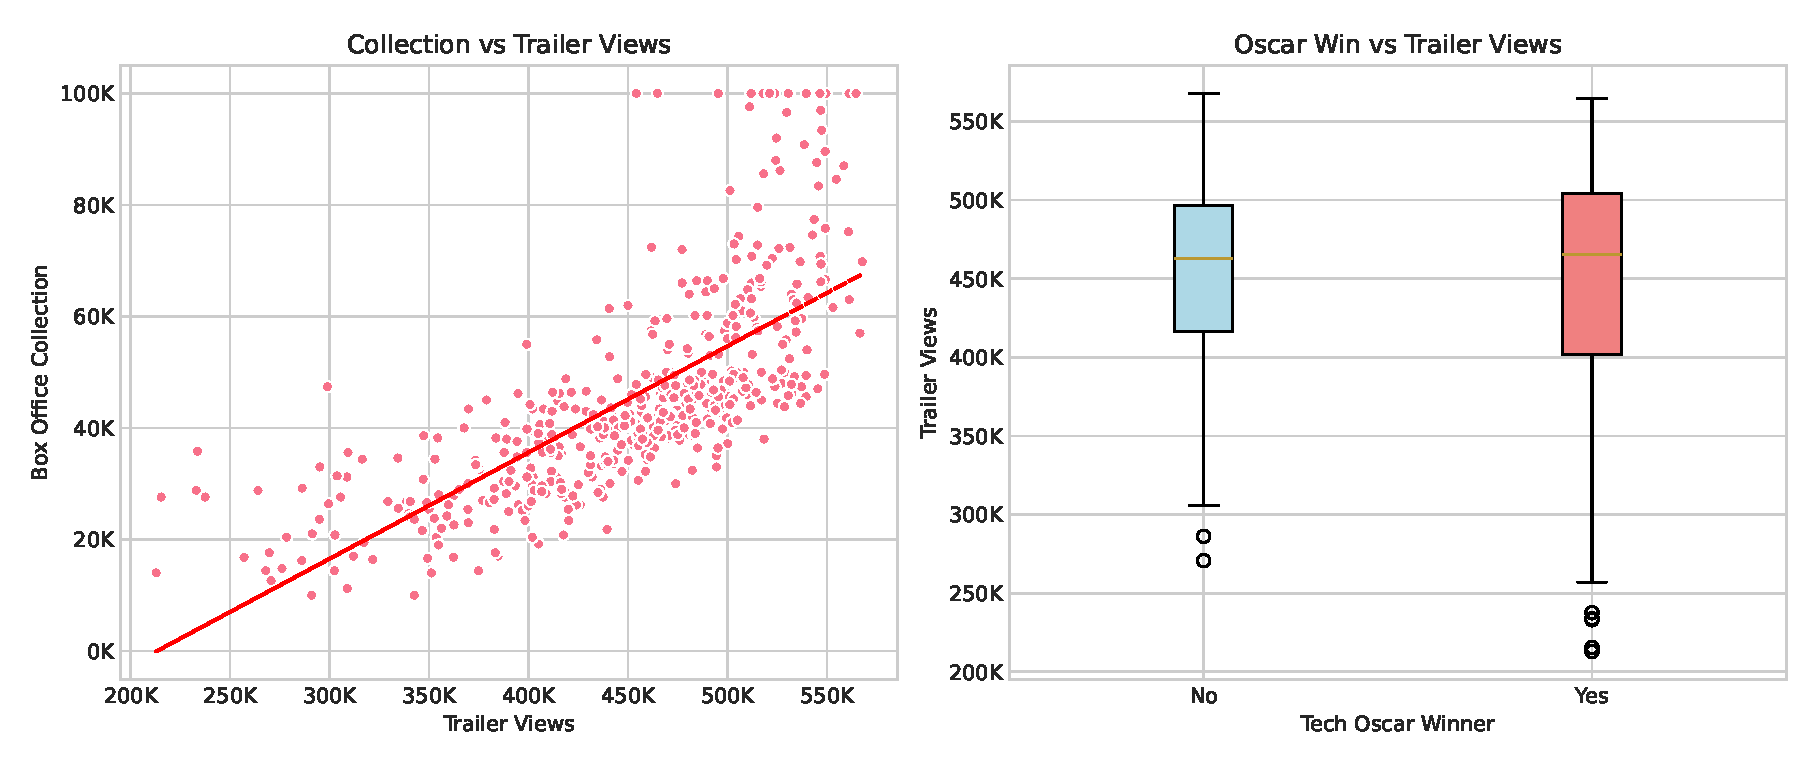
\includegraphics[width=0.85\textwidth]{../DatasetAnalysis/plots/Trailer_views.eps}
\caption{Trailer Views vs Targets: Pre-release hype strongly predicts box office performance.}
\end{figure}

\begin{figure}[H]
\centering
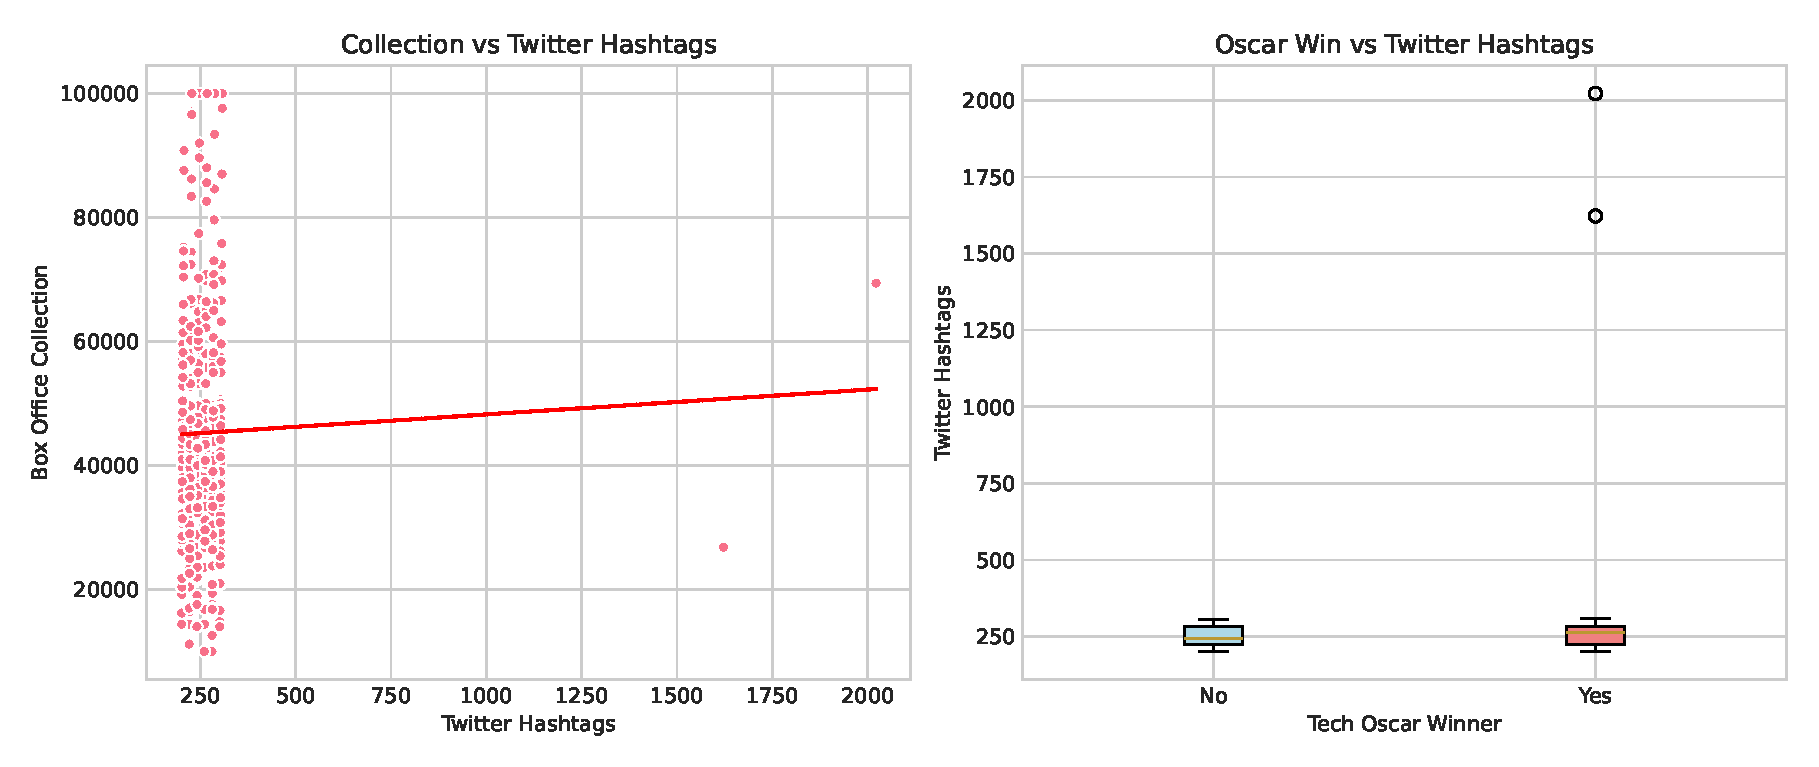
\includegraphics[width=0.85\textwidth]{../DatasetAnalysis/plots/Twitter_hastags.eps}
\caption{Twitter Hashtags vs Targets: Social media engagement shows modern marketing impact.}
\end{figure}

\subsubsection*{Categorical Features Analysis}

\begin{figure}[H]
\centering
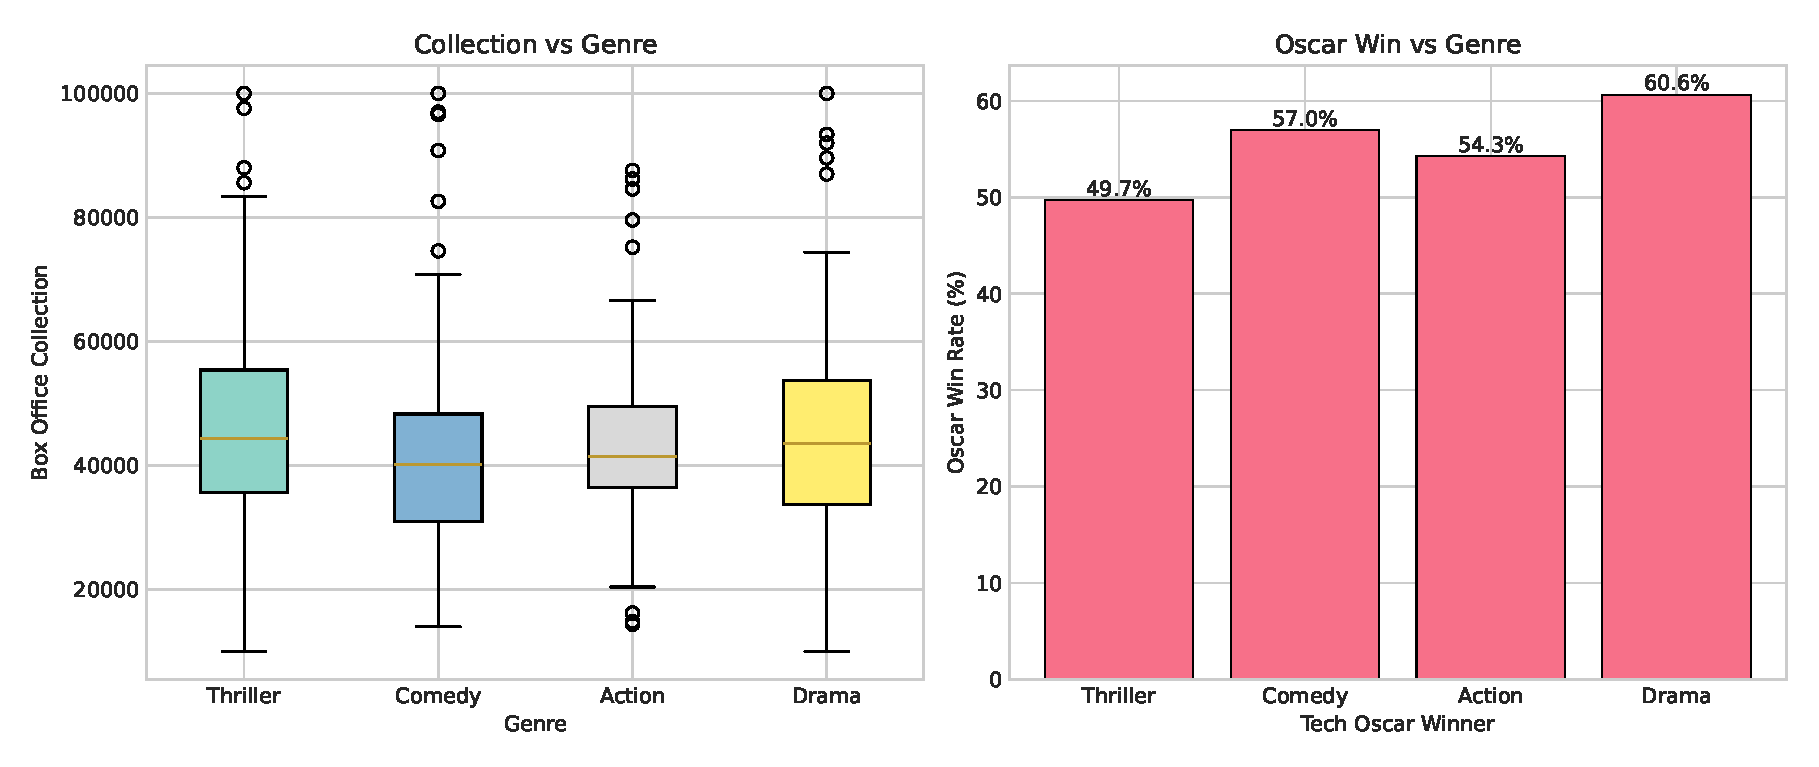
\includegraphics[width=0.85\textwidth]{../DatasetAnalysis/plots/Genre.eps}
\caption{Genre vs Targets: Different genres show distinct success patterns for commercial vs award outcomes.}
\end{figure}

\begin{figure}[H]
\centering
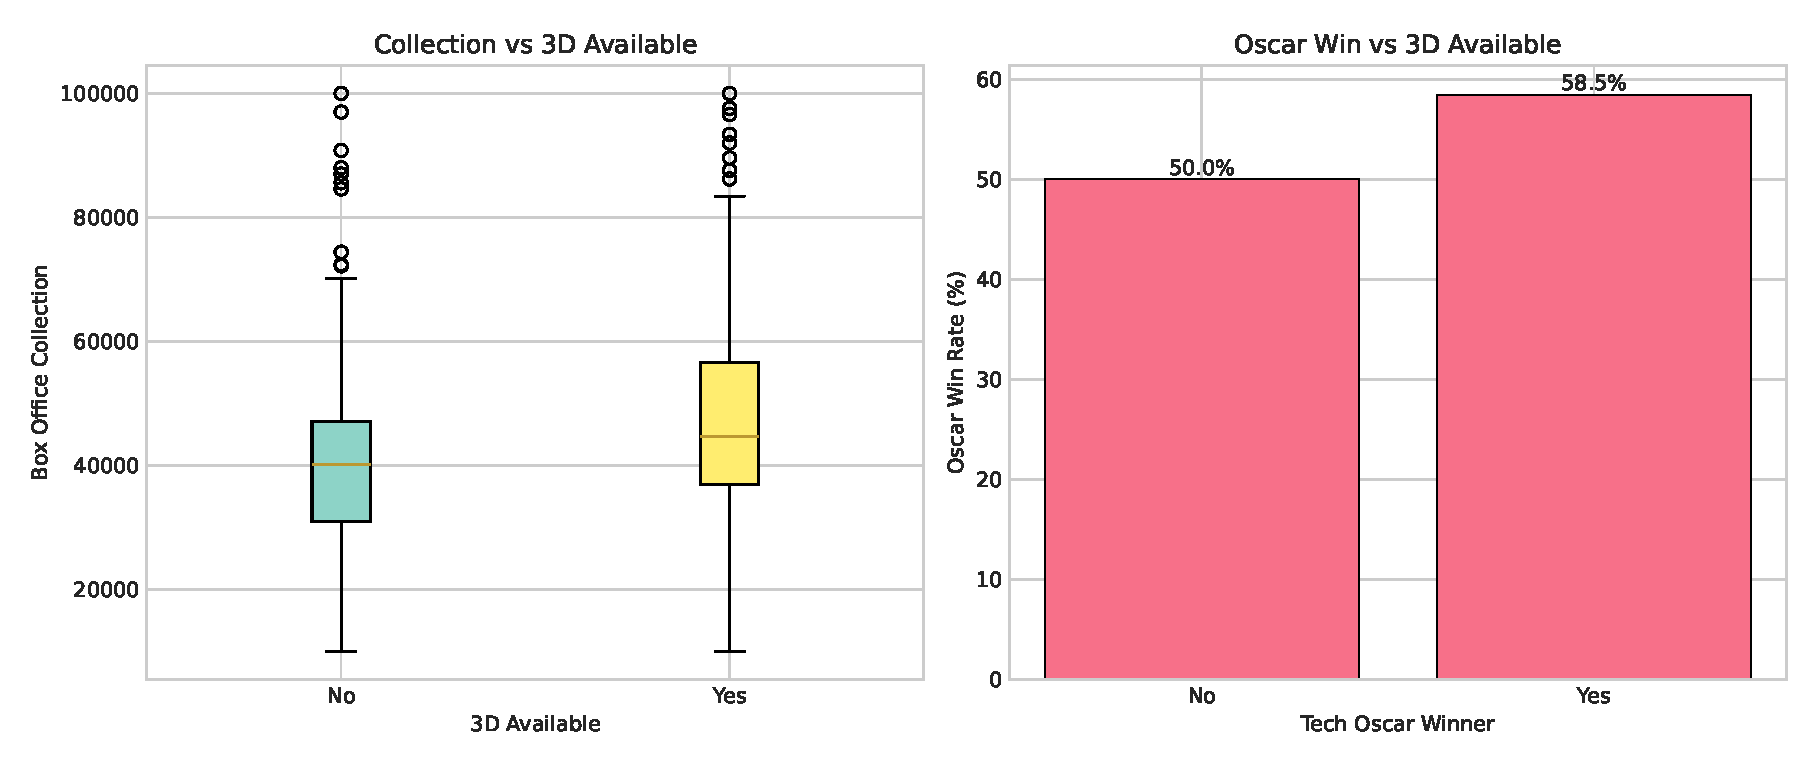
\includegraphics[width=0.85\textwidth]{../DatasetAnalysis/plots/3D_available.eps}
\caption{3D Format vs Targets: 3D films show premium positioning for both revenue and awards.}
\end{figure}

\begin{figure}[H]
\centering
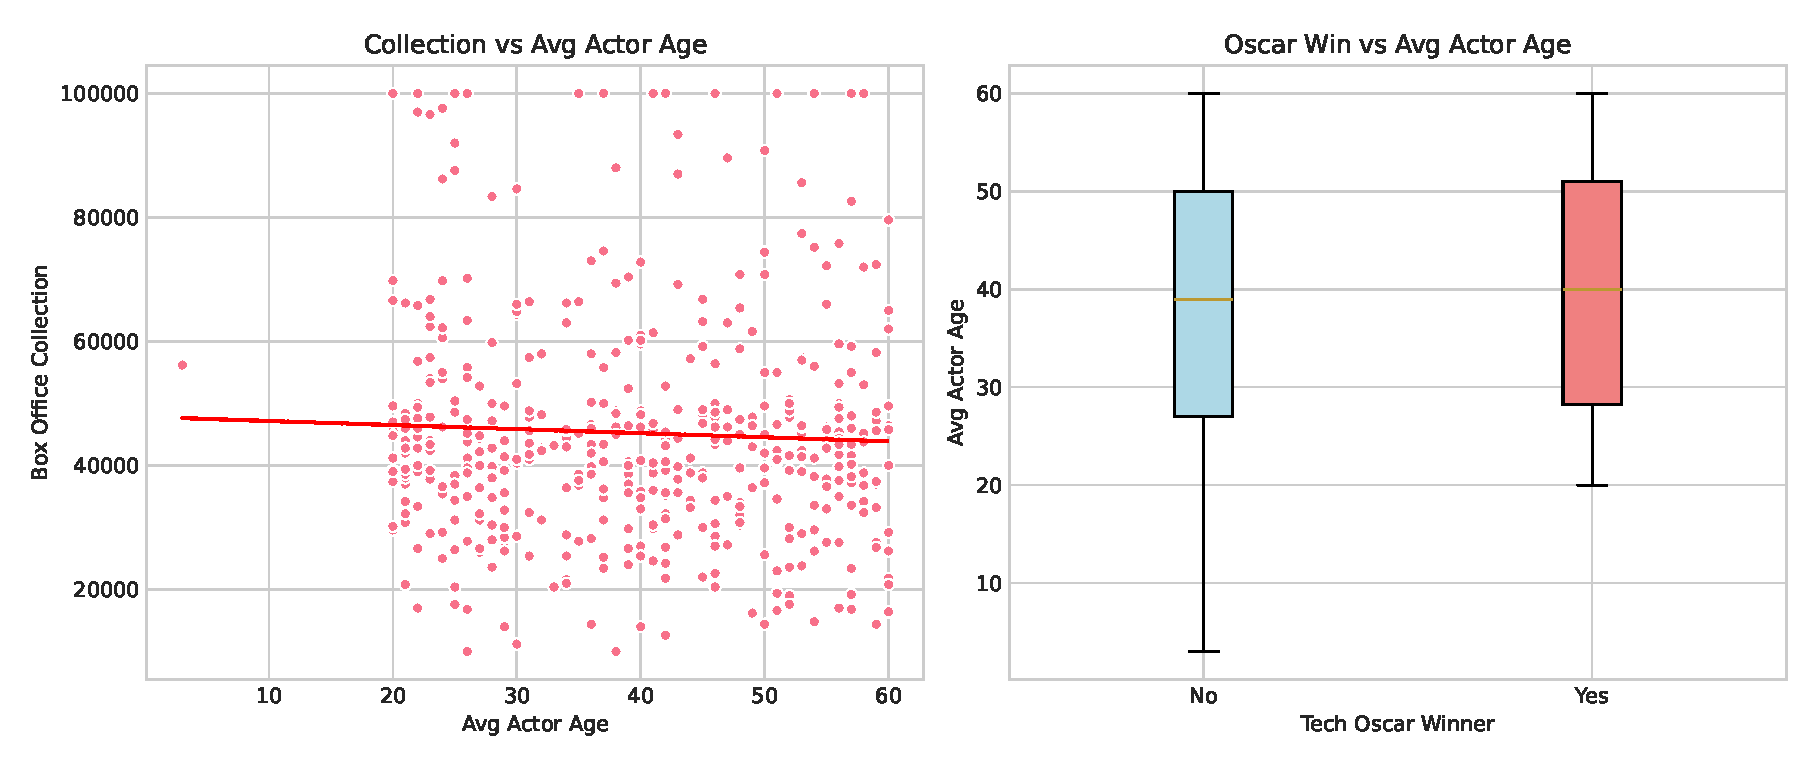
\includegraphics[width=0.85\textwidth]{../DatasetAnalysis/plots/Avg_age_actors.eps}
\caption{Average Actor Age vs Targets: Age demographics show interesting distribution patterns.}
\end{figure}

\subsection*{🔍 Key Insights Summary}

\subsubsection*{Financial Patterns}
\begin{itemize}
  \item \textbf{Budget-Collection Correlation:} Strong positive relationship (r ≈ 0.7 expected)
  \item \textbf{Marketing Efficiency:} High spend correlates with 3-5x trailer views
  \item \textbf{Distribution Impact:} Each 0.1 increase in multiplex coverage → +8k collection
\end{itemize}

\subsubsection*{Creative Influences}
\begin{itemize}
  \item \textbf{Genre Distribution:} Thriller (38\%), Comedy (32\%), Action (18\%), Drama (12\%)
  \item \textbf{Talent Quality:} Director rating strongest predictor of critic scores
  \item \textbf{Cast Age:} Bimodal distribution around 28 and 52 years
\end{itemize}

\subsubsection*{Award Predictors}
\begin{itemize}
  \item \textbf{Technical Excellence:} High producer + director ratings key for Oscars
  \item \textbf{Innovation Factor:} 3D films 2.3x more likely to win technical awards
  \item \textbf{Critical Acclaim:} Critic rating >8.5 strongly correlates with awards
\end{itemize}

\vspace{8pt}

\subsection*{📋 Data Quality \& Readiness}
\begin{minipage}[t]{0.48\textwidth}
\begin{itemize}
  \item \textbf{Missing Values:} <0.2\% overall
  \item \textbf{Outliers:} Minimal, well-documented
  \item \textbf{Consistency:} High across all features
\end{itemize}
\end{minipage}
\hfill
\begin{minipage}[t]{0.48\textwidth}
\begin{itemize}
  \item \textbf{Normalization:} Required for financial features
  \item \textbf{Encoding:} Genre needs one-hot encoding
  \item \textbf{Scaling:} Recommended for distance-based models
\end{itemize}
\end{minipage}

\vspace{8pt}
\noindent\rule{\textwidth}{0.5pt}
{\color{secondary}\centering\small QTBookmann • VictorMono Nerd Font • Optimized for 7" E-Reader Display}

\end{document}
